%!TEX root = main.tex 


\section{Design Overview} 
\label{sec:overview} 

\noindent Building upon the aforementioned observations and motivations, 
we introduce \sys, a simulator tailored for large-scale LLM training.

\begin{comment}
\vspace{0.2em}
\noindent\textbf{Design objective.}
A performance simulator should predict the step time of a training model with minimal effort while providing high-quality runtime statistics for each stage of the training process. Our primary objective is to design an accurate simulator that reduces the need for repetitive and costly experiments. We focus on large-scale distributed training for two key reasons: (1) Large-scale training is particularly expensive, and we expect that \sys can significantly reduce costs. (2) Large-scale distributed training often experiences greater performance degradation due to device communication, making it more challenging to identify bottlenecks and optimize efficiency.
\end{comment}

\noindent\textbf{Key design choices.}
% \hxq{highlight and explain the key design choices of \sys.}
We highlight the key choices in building \sys to address the three challenges in \cref{subsec:challenges}. 
% previous methods for extracting training workloads typically involve either running on physical clusters (trace-based approaches) or incurring significant manual labor (manual-based approaches). 
\begin{itemize}[leftmargin=*]

\item To obtain training workloads without a full-scale deployment, \sys employs a novel ex-situ tracing approach. 
Generally, ML frameworks support various parallelism in the following way: (1) they initialize each rank (typically one rank per device) with its own sub-model based on the parallelism setting, and then (2) each rank builds its own execution graph to start actual training. 
\sys turns this parallel process into a sequential one, using only one device to act as each rank iteratively to trace the corresponding execution graph and profile the running time of each \op at the same time, achieving faithful workload tracing without requiring the full cluster.

% \sys strikes a balance between these extremes by developing a generalized tracer, compatible with mainstream training frameworks such as DeepSpeed, and Megatron-LM. While our approach (\cref{sec:workload_const_replay}) remains trace-driven to ensure the precision of \wg{}s, it eliminates the resource constraints of traditional methods, allowing users to capture distributed training workloads from a single standard GPU, significantly reducing the cost of workload extraction.

\item To achieve accurate and efficient communication simulation, \sys employs a white-box modeling approach with empirically profiled parameters that strikes a good balance between accuracy and efficiency.
% This compromise involves constructing a generalized formulation of the communication process 
Our model is derived closely after NCCL's underlying chunk-based implementation of collective communication capturing critical factors such as per-chunk inter-server transmission time. 
These factors are profiled offline exhaustively to capture the complex dynamic optimization by \nccl according to hardware features and software configurations.

\item To account for the interference between overlapping computation and communication, \sys adopts a black-box method using features related to both computation and communication kernels, such as bucket size, SM occupancy, and cache hit rate.
\end{itemize}
% The model is trained using kernel performance data from single-device runs and the parameters of communication setting to predict their interaction and resulting slowdown.
% \hxq{merge this with the overall arch}
% \noindent\textbf{System input.}
% \sys requires three inputs: (1) User variable: This describe the selected training framework (e.g., PyTorch, DeepSpeed, Megatron-LM), training strategy details (e.g., 3D parallelism, overlap), and simulation settings such as profiling scope and iteration count. (2) Model configuration: This includes model settings such as structure, hyperparameters (e.g., hidden size, number of layers, bucket size). (3) Hardware configuration: This specifies the physical cluster setup, including cluster size, network topology (both intra- and inter-server), and NCCL environment parameters (e.g. NCCL\_TOPO\_FILE, NCCL\_BUFFSIZE).


% \vspace{0.2em}
% \noindent\textbf{System architecture.} 
% Figure~\ref{fig:arch} illustrates the architecture of \sys.
% The \textit{\extractor} constructs the training workload using tailored modules for tracing \wg. 
% It generates detailed workload information, including computation and meta-information for communication workloads, using an enhanced tracing approach, and performs quick GPU memory checks to validate the training plan (i.e., out-off-memory check). The \textit{\cm} predicts the runtime of communication kernels (\cref{sec:comm_pred}). It includes a network performance benchmarking module optimized for NCCL, capable of formulating communication functions based on the profiled dataset. The \textit{\ma} replays the training process (\cref{subsec:workload_replay}). It reorganizes the execution sub-graphs of all GPUs and schedules the operators in global timelines, accurately simulating the training behavior. The \textit{\va} adjusts the runtime of overlapped kernels based on a ML approach to reflect slowdown inferences (\cref{sec:overlap_pred}). Additionally, \sys embeds a \textit{database} to store and share profiling data, facilitating predictions and reducing redundant profiling.

% \fx{hx:merge this with the overall arch}
\noindent\textbf{System architecture.}
Figure~\ref{fig:arch} shows \sys's architecture.
Its input includes three categories: user-defined settings specifying the training framework, parallelism strategies (DP/TP/PP/EP groups); model details defining the model structure and hyperparameters; and hardware configurations detailing device specifics (GPU type), cluster size, network topology, \nccl parameters (e.g., NCCL\_TOPO\_FILE, NCCL\_BUFFSIZE), etc.
Given these inputs, the \textit{\extractor} extracts training workloads for each rank, including the per-rank execution graph and \op running times (\cref{subsec:workload_const}). 
% It employs an enhanced tracing approach to generate detailed computation and communication workloads, and performs quick memory checks to detect insufficient memory conditions, reporting out-of-memory errors when necessary.
The \textit{\cm} module (\cref{sec:comm_pred}) leverages the white-box models with parameters corresponding to the given settings to estimate each communication kernel's performance. 
Then the \textit{\ma} module (\cref{subsec:workload_replay}) re-constructs the global timelines of the end-to-end training process by assembling all per-rank execution graphs with estimated communication \op performance and inter-rank dependencies. 
The \textit{\va} module (\cref{sec:overlap_pred}) applies a machine learning model to adjust the running times of overlapping operations, accounting for the interference-induced slowdown, and outputs the final training step time result.  
Additionally, \sys maintains a \textit{database} for profiling data, reducing redundant measurements across simulations.

% \noindent\textbf{System workflow.} 
% \sys begins by analyzing the provided inputs.
% The \textit{\extractor} then loads the model on a single GPU to derive execution sub-graphs for all devices involved iteratively. If a requested operation's profile is not already in the database, \sys profiles it and stores the result. For communication operations, the \textit{\cm} uses the profiled data based on a white-box approach to predict their runtimes. Once all sub-graphs are collected, the \textit{\ma} arranges them in global timelines. When operations overlap, the \textit{\va} adjusts their runtimes to reflect realistic slowdowns. Finally, \sys produces a comprehensive performance report.


\begin{figure}[t] 
    \centering 
    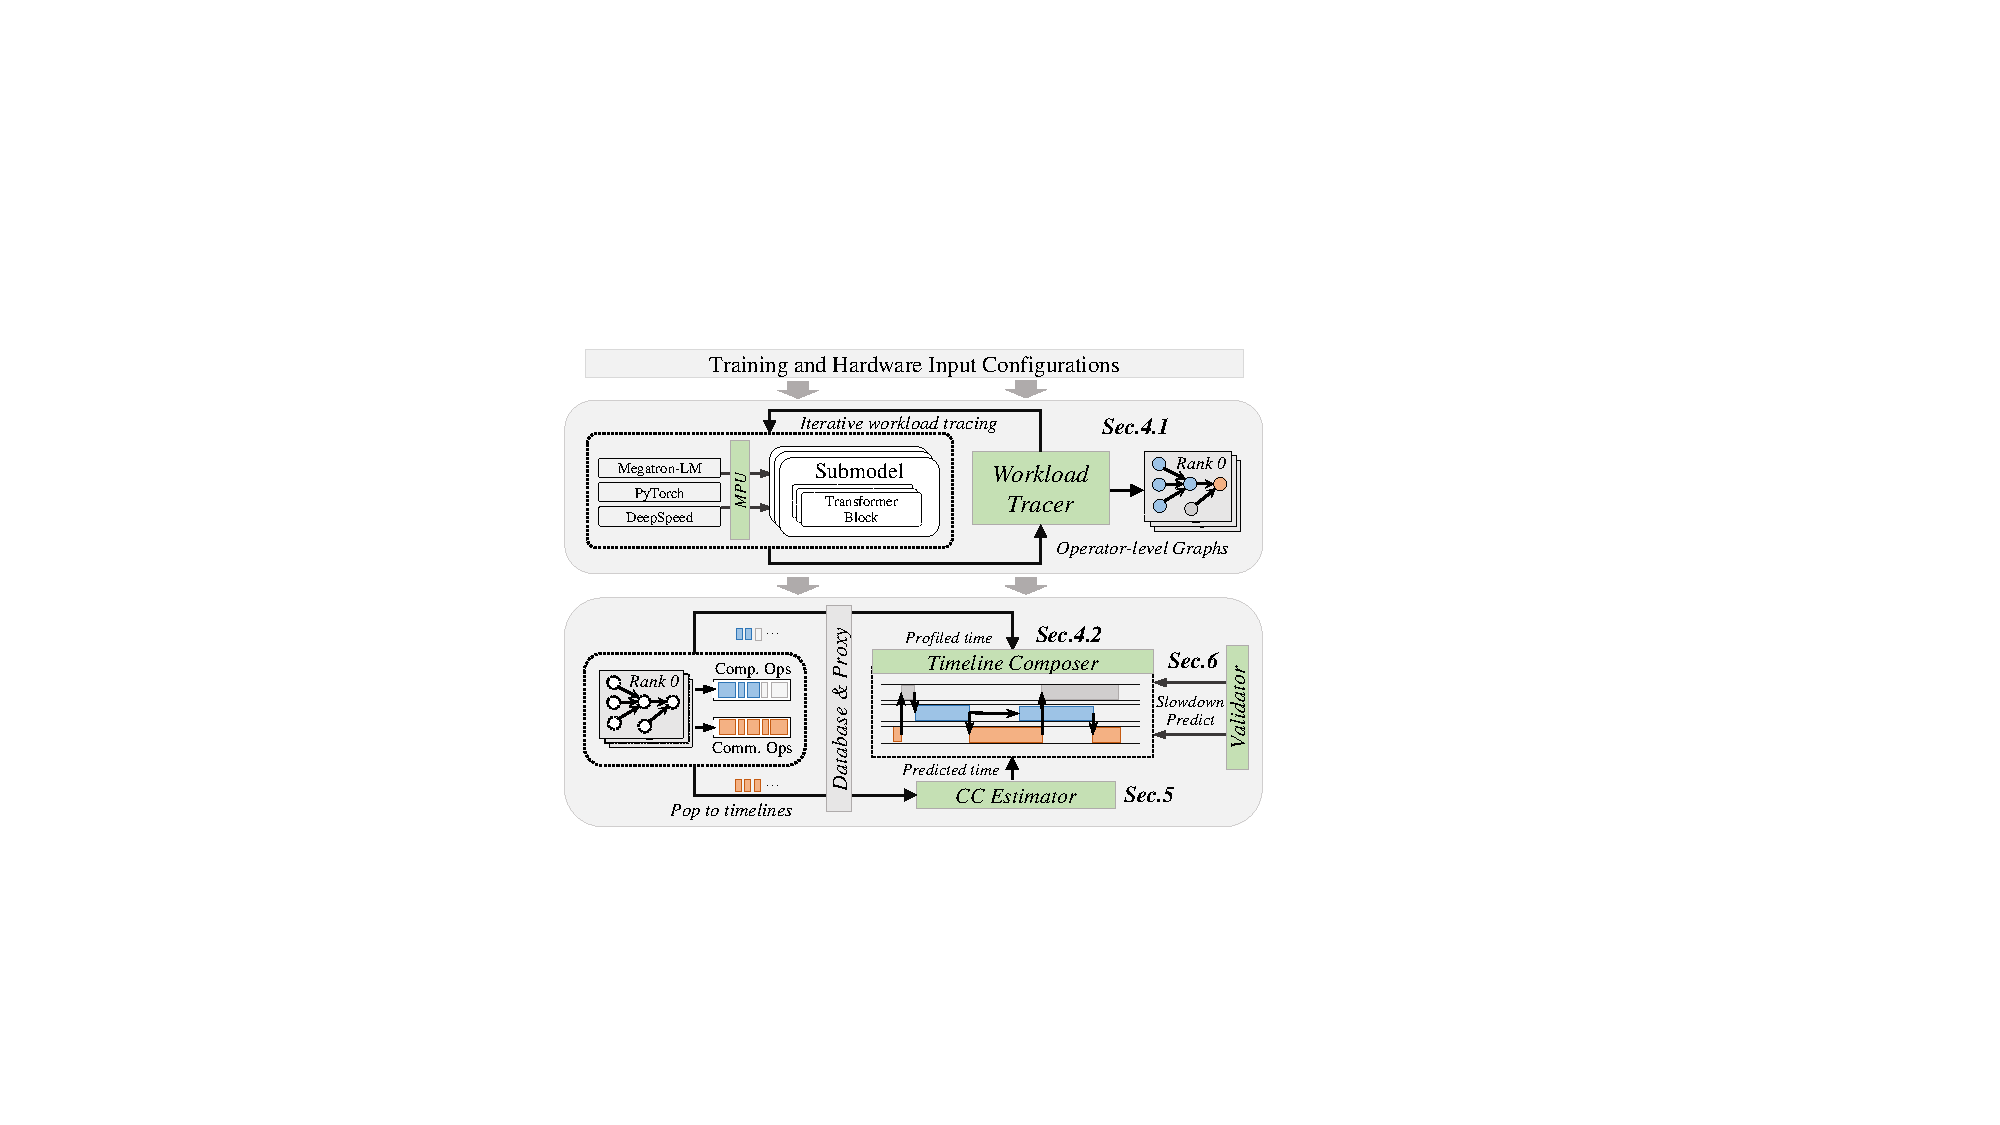
\includegraphics[width=\linewidth]{figures/design/moye_overview.pdf} 
    \caption{\sys architecture overview. The green components represent the core modules of \sys.} 
    \label{fig:arch} 
    \vspace{-1.5em}
\end{figure}



% In \sys, we center around two key questions: 
% \begin{itemize}[leftmargin=3mm] 
%     \item How to accurately estimate the all-reduce running time given a large-scale cluster configuration? 
%     \item How to predict the slowdown factor of kernels that are interfered by the concurrent all-reduce kernel? 
% \end{itemize}

